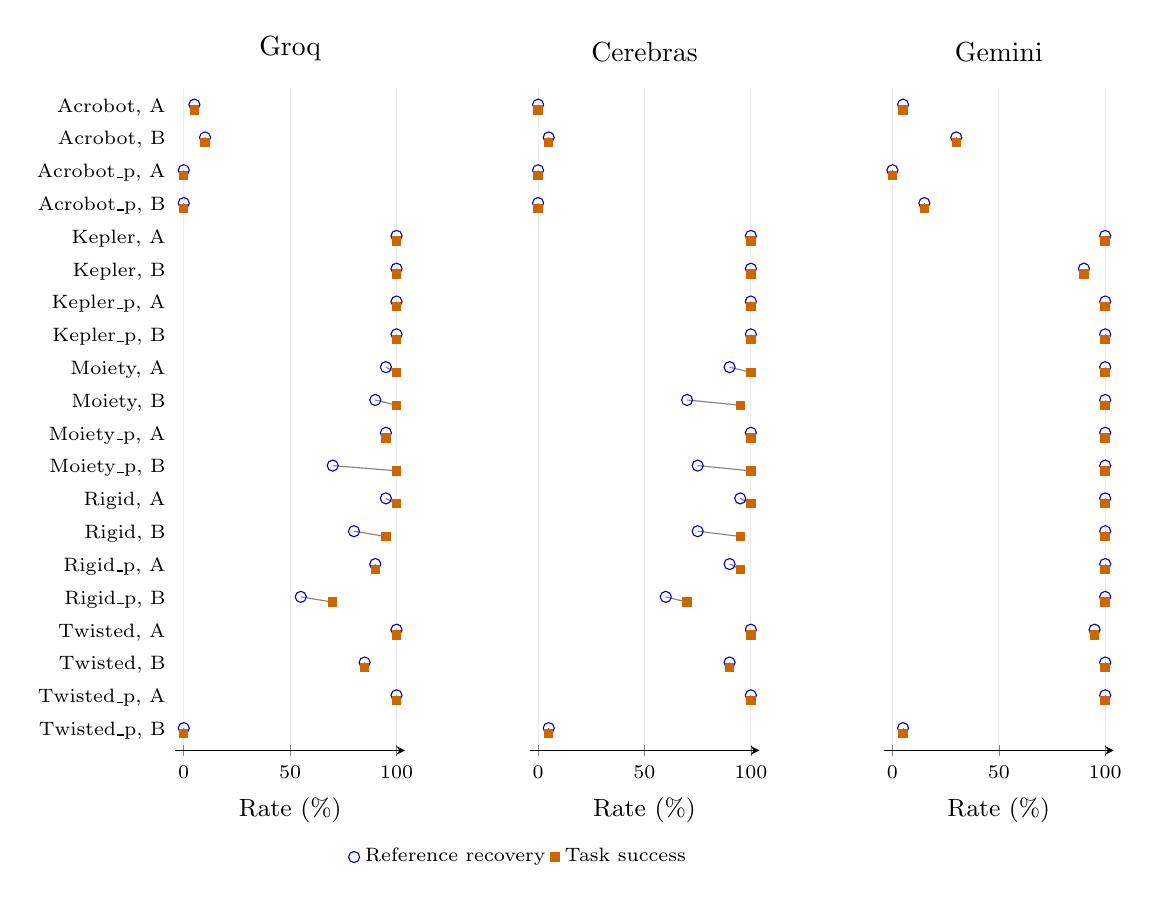
\begin{tikzpicture}
\begin{axis}[at={(0.0cm,0)},anchor=west,width=4.5cm,height=10cm,xmin=-4,xmax=104,ymin=0.4,ymax=20.6,xtick={0,50,100},xlabel={Rate (\%)},ytick={20,19,18,17,16,15,14,13,12,11,10,9,8,7,6,5,4,3,2,1},yticklabels={{Acrobot, A},{Acrobot, B},{Acrobot\_p, A},{Acrobot\_p, B},{Kepler, A},{Kepler, B},{Kepler\_p, A},{Kepler\_p, B},{Moiety, A},{Moiety, B},{Moiety\_p, A},{Moiety\_p, B},{Rigid, A},{Rigid, B},{Rigid\_p, A},{Rigid\_p, B},{Twisted, A},{Twisted, B},{Twisted\_p, A},{Twisted\_p, B}},tick label style={font=\scriptsize},label style={font=\small},xmajorgrids=true,grid style={gray!15},axis y line*=left,axis x line=bottom,y axis line style={draw=none},ytick style={draw=none},title={Groq},legend style={font=\scriptsize,draw=none,at={(1.5,-0.13)},anchor=north,legend columns=2}]
\addplot[gray,thin,unbounded coords=jump] coordinates {(5,20.08) (5,19.92) (nan,nan) (10,19.08) (10,18.92) (nan,nan) (0,18.08) (0,17.92) (nan,nan) (0,17.08) (0,16.92) (nan,nan) (100,16.08) (100,15.92) (nan,nan) (100,15.08) (100,14.92) (nan,nan) (100,14.08) (100,13.92) (nan,nan) (100,13.08) (100,12.92) (nan,nan) (95,12.08) (100,11.92) (nan,nan) (90,11.08) (100,10.92) (nan,nan) (95,10.08) (95,9.92) (nan,nan) (70,9.08) (100,8.92) (nan,nan) (95,8.08) (100,7.92) (nan,nan) (80,7.08) (95,6.92) (nan,nan) (90,6.08) (90,5.92) (nan,nan) (55,5.08) (70,4.92) (nan,nan) (100,4.08) (100,3.92) (nan,nan) (85,3.08) (85,2.92) (nan,nan) (100,2.08) (100,1.92) (nan,nan) (0,1.08) (0,0.92) (nan,nan)};
\addplot[only marks,mark=o,blue!75!black] coordinates {(5,20.08) (10,19.08) (0,18.08) (0,17.08) (100,16.08) (100,15.08) (100,14.08) (100,13.08) (95,12.08) (90,11.08) (95,10.08) (70,9.08) (95,8.08) (80,7.08) (90,6.08) (55,5.08) (100,4.08) (85,3.08) (100,2.08) (0,1.08)};
\addplot[only marks,mark=square*,mark size=1.5pt,orange!80!black] coordinates {(5,19.92) (10,18.92) (0,17.92) (0,16.92) (100,15.92) (100,14.92) (100,13.92) (100,12.92) (100,11.92) (100,10.92) (95,9.92) (100,8.92) (100,7.92) (95,6.92) (90,5.92) (70,4.92) (100,3.92) (85,2.92) (100,1.92) (0,0.92)};
\legend{,Reference recovery,Task success}
\end{axis}
\begin{axis}[at={(4.5cm,0)},anchor=west,width=4.5cm,height=10cm,xmin=-4,xmax=104,ymin=0.4,ymax=20.6,xtick={0,50,100},xlabel={Rate (\%)},ytick={20,19,18,17,16,15,14,13,12,11,10,9,8,7,6,5,4,3,2,1},yticklabels={},tick label style={font=\scriptsize},label style={font=\small},xmajorgrids=true,grid style={gray!15},axis y line*=left,axis x line=bottom,y axis line style={draw=none},ytick style={draw=none},title={Cerebras},legend style={font=\scriptsize,draw=none,at={(1.5,-0.13)},anchor=north,legend columns=2}]
\addplot[gray,thin,unbounded coords=jump] coordinates {(0,20.08) (0,19.92) (nan,nan) (5,19.08) (5,18.92) (nan,nan) (0,18.08) (0,17.92) (nan,nan) (0,17.08) (0,16.92) (nan,nan) (100,16.08) (100,15.92) (nan,nan) (100,15.08) (100,14.92) (nan,nan) (100,14.08) (100,13.92) (nan,nan) (100,13.08) (100,12.92) (nan,nan) (90,12.08) (100,11.92) (nan,nan) (70,11.08) (95,10.92) (nan,nan) (100,10.08) (100,9.92) (nan,nan) (75,9.08) (100,8.92) (nan,nan) (95,8.08) (100,7.92) (nan,nan) (75,7.08) (95,6.92) (nan,nan) (90,6.08) (95,5.92) (nan,nan) (60,5.08) (70,4.92) (nan,nan) (100,4.08) (100,3.92) (nan,nan) (90,3.08) (90,2.92) (nan,nan) (100,2.08) (100,1.92) (nan,nan) (5,1.08) (5,0.92) (nan,nan)};
\addplot[only marks,mark=o,blue!75!black] coordinates {(0,20.08) (5,19.08) (0,18.08) (0,17.08) (100,16.08) (100,15.08) (100,14.08) (100,13.08) (90,12.08) (70,11.08) (100,10.08) (75,9.08) (95,8.08) (75,7.08) (90,6.08) (60,5.08) (100,4.08) (90,3.08) (100,2.08) (5,1.08)};
\addplot[only marks,mark=square*,mark size=1.5pt,orange!80!black] coordinates {(0,19.92) (5,18.92) (0,17.92) (0,16.92) (100,15.92) (100,14.92) (100,13.92) (100,12.92) (100,11.92) (95,10.92) (100,9.92) (100,8.92) (100,7.92) (95,6.92) (95,5.92) (70,4.92) (100,3.92) (90,2.92) (100,1.92) (5,0.92)};
\end{axis}
\begin{axis}[at={(9.0cm,0)},anchor=west,width=4.5cm,height=10cm,xmin=-4,xmax=104,ymin=0.4,ymax=20.6,xtick={0,50,100},xlabel={Rate (\%)},ytick={20,19,18,17,16,15,14,13,12,11,10,9,8,7,6,5,4,3,2,1},yticklabels={},tick label style={font=\scriptsize},label style={font=\small},xmajorgrids=true,grid style={gray!15},axis y line*=left,axis x line=bottom,y axis line style={draw=none},ytick style={draw=none},title={Gemini},legend style={font=\scriptsize,draw=none,at={(1.5,-0.13)},anchor=north,legend columns=2}]
\addplot[gray,thin,unbounded coords=jump] coordinates {(5,20.08) (5,19.92) (nan,nan) (30,19.08) (30,18.92) (nan,nan) (0,18.08) (0,17.92) (nan,nan) (15,17.08) (15,16.92) (nan,nan) (100,16.08) (100,15.92) (nan,nan) (90,15.08) (90,14.92) (nan,nan) (100,14.08) (100,13.92) (nan,nan) (100,13.08) (100,12.92) (nan,nan) (100,12.08) (100,11.92) (nan,nan) (100,11.08) (100,10.92) (nan,nan) (100,10.08) (100,9.92) (nan,nan) (100,9.08) (100,8.92) (nan,nan) (100,8.08) (100,7.92) (nan,nan) (100,7.08) (100,6.92) (nan,nan) (100,6.08) (100,5.92) (nan,nan) (100,5.08) (100,4.92) (nan,nan) (95,4.08) (95,3.92) (nan,nan) (100,3.08) (100,2.92) (nan,nan) (100,2.08) (100,1.92) (nan,nan) (5,1.08) (5,0.92) (nan,nan)};
\addplot[only marks,mark=o,blue!75!black] coordinates {(5,20.08) (30,19.08) (0,18.08) (15,17.08) (100,16.08) (90,15.08) (100,14.08) (100,13.08) (100,12.08) (100,11.08) (100,10.08) (100,9.08) (100,8.08) (100,7.08) (100,6.08) (100,5.08) (95,4.08) (100,3.08) (100,2.08) (5,1.08)};
\addplot[only marks,mark=square*,mark size=1.5pt,orange!80!black] coordinates {(5,19.92) (30,18.92) (0,17.92) (15,16.92) (100,15.92) (90,14.92) (100,13.92) (100,12.92) (100,11.92) (100,10.92) (100,9.92) (100,8.92) (100,7.92) (100,6.92) (100,5.92) (100,4.92) (95,3.92) (100,2.92) (100,1.92) (5,0.92)};
\end{axis}
\end{tikzpicture}
